% Prepared by Edwin Mugume, PhD - Department of Electrical and Computer Engineering, Makerere University
% Official template for NCC 2026 which is based on the IEEEtran class (11pt)
% Paper 83: OptiscanAI — Large Vision Models for Multi-Disease Retinal Screening in Ugandan Healthcare

\documentclass[11pt]{IEEEtran}
\usepackage{graphicx}
\usepackage{amsmath}
\usepackage{amssymb}
\usepackage{flushend}
\usepackage{balance}
\usepackage{booktabs}
\usepackage{url}
\usepackage[hidelinks]{hyperref}

\graphicspath{{figs/}}

\title{OptiscanAI: Large Vision Models for Multi-Disease Retinal Screening in Ugandan Healthcare\\A Benchmark and Deployment Study}

\author{
    \IEEEauthorblockN{Lauben Mpairwe\IEEEauthorrefmark{1}, Shadia Nankya\IEEEauthorrefmark{1},
    Rebecca Yapyeko\IEEEauthorrefmark{1}, Marvin Ggaliwango\IEEEauthorrefmark{2}}
    \\\IEEEauthorblockA{\IEEEauthorrefmark{1} Department of Networks, College of Computing and
    Information Sciences \\ Makerere University, Kampala, Uganda \\
    Email: \{mpairwe\_lauben, nankya.shadia, yapyeko.rebecca\}@students.mak.ac.ug}
    \\\IEEEauthorblockA{\IEEEauthorrefmark{2} Department of Computer Science, College of Computing and Information Sciences \\ Makerere
    University, Kampala, Uganda \\ Email: ggaliwango.marvin@cit.ac.ug}
}

\begin{document}

\maketitle

\begin{abstract}
Preventable blindness from vitreoretinal and optic nerve pathologies presents a critical global
burden, exacerbated by the acute shortage of specialist ophthalmologists across sub-Saharan Africa.
This investigation delivers a rigorous empirical assessment of OptiscanAI, an integrated multi-label
retinal screening framework adapted from a domain-specific foundation model, evaluated strictly on the
held-out official test partition (640 images) of the Retinal Fundus Multi-Disease Image Dataset. We
detail class-stratified sensitivity, specificity, positive predictive value (PPV), false-negative rate,
and area under the precision-recall curve (AUPRC) with 95\% bootstrap confidence intervals, alongside
controlled ablations across network backbones, parameter-efficient adaptation, and dynamic 8-bit
quantization. Our findings illuminate three operational realities for low-resource translation. First,
discriminative capacity is robust yet unevenly distributed: macro AUC reaches 0.872, ranging from
0.996 for myopia to 0.663 for optic disc pallor. Second, uncalibrated probability outputs exhibit
severe over-confidence (expected calibration error 0.209), causing static decision thresholds to
silence five diagnostic channels; isotonic recalibration mitigates this error to 0.003 without
altering discriminative ranking. Third, while binary referral triage achieves an AUC of 0.952,
projecting this operating point to primary-care clinical prevalence drops PPV from 0.93 to below
0.30. Consequently, we articulate these findings as rigorous benchmark evidence and infrastructural
feasibility analyses rather than clinical validation within Uganda.
\end{abstract}

\begin{IEEEkeywords}
retinal screening, multi-label classification, model calibration, explainability, low-resource
deployment, foundation models
\end{IEEEkeywords}

\section{Introduction}

Preventable blindness represents an escalating healthcare crisis: the World Health Organization
estimates that 2.2 billion individuals endure visual impairment, over half treatable if diagnosed
early~\cite{who2019}. Microvascular complications such as diabetic retinopathy affected over
103 million patients by 2020 and continue to expand in developing regions~\cite{teo2021}. In Uganda,
specialist ophthalmologists are concentrated in urban referral centres, leaving non-specialist
primary healthcare workers as the initial gatekeepers for ocular screening. Under these constraints,
insidious pathologies---such as diabetic retinopathy, hypertensive remodeling, and glaucomatous
neuropathy---are frequently missed until irreversible vision loss occurs.

Although deep neural models achieve high diagnostic accuracy on isolated conditions~\cite{gulshan2016},
and retinal foundation backbones exhibit versatile transfer~\cite{retfound2023}, practical deployment
in resource-constrained clinics faces critical challenges: severe class skew, clinical explainability
demands, unstable telecommunications, and population distribution shift~\cite{beede2020,wiens2019}.

In response to peer review of our initial report, this manuscript addresses the core concerns raised.
Reviewers correctly observed that evaluation on an international benchmark (RFMiD) cannot support
unqualified clinical claims in Ugandan healthcare, and requested explicit disentanglement of component
contributions. We retain the system architecture but reposition our claims: what follows is benchmark
evidence and deployment-constraint analysis, stating the gap to clinical readiness quantitatively rather
than as a caveat.

\textbf{Contributions.} (i) A per-disease evaluation on the held-out RFMiD test split reporting
sensitivity, specificity, PPV, FNR, and AUPRC with 95\% bootstrap confidence intervals. (ii) A unified
ablation isolating retinal pretraining, LoRA adaptation, decision thresholding, and INT8 quantization
under a shared training recipe. (iii) Diagnosis of a calibration failure that silences five disease
channels, with a rank-preserving correction. (iv) Quantitative faithfulness testing of saliency maps
and generated text via insertion/deletion metrics. (v) A prevalence-transfer model mapping benchmark
triage metrics onto primary-care referral burdens.

\section{Related Work}

\subsection{Retinal Detection and Foundation Models}
Deep learning for retinal fundus analysis was established by Gulshan \emph{et al.}~\cite{gulshan2016}
for diabetic retinopathy, and extended to glaucoma and macular degeneration, predominantly on single-disease
tasks. Frontline screening requires multi-label classification across heterogeneous taxonomies, where class
imbalance, co-morbidity, and positive scarcity impede learning~\cite{rfmid2021}. Vision
Transformers~\cite{vit2021} capture global spatial dependencies across fundus patches, and RETFound~\cite{retfound2023},
pretrained on 1.6 million retinal images, surpasses ImageNet initialisation on ophthalmic benchmarks.
Low-Rank Adaptation (LoRA)~\cite{lora2022} updates parameter subspaces while freezing backbone weights,
enabling adaptation under constrained compute budgets.

\subsection{Imbalance, Calibration and Explainability}
Asymmetric~\cite{asl2021} and focal losses~\cite{focal2017} address imbalance by down-weighting easy
negatives, but can distort probability calibration in over-confident networks~\cite{guo2017}; recalibration
via Platt scaling restores usable probabilities while preserving ranking. Grad-CAM~\cite{gradcam2017} and
Integrated Gradients~\cite{ig2017} are standard attribution baselines, evaluated via perturbation
metrics~\cite{rise2018}. Field studies confirm that workflow ergonomics, image quality, and clinician trust
dominate real-world effectiveness~\cite{beede2020}.

\section{System Architecture}

Fig.~\ref{fig:arch} shows the pipeline; the numbers below refer to its labelled components.

\begin{figure*}[!t]
    \centering
    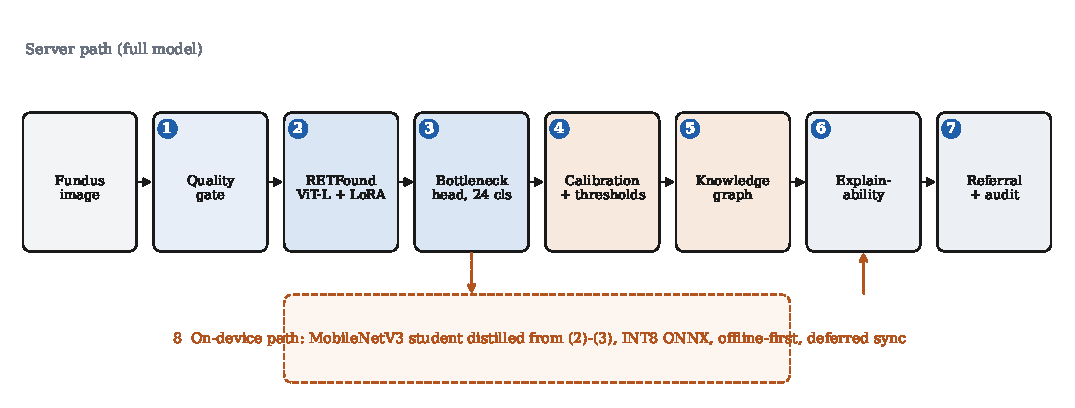
\includegraphics[width=\textwidth]{fig1_architecture.pdf}
    \caption{OptiscanAI pipeline. (1) image quality gate; (2) RETFound ViT-L/16 backbone with
    LoRA adapters; (3) bottleneck classification head over 24 retained classes; (4) probability
    calibration and per-class decision thresholds; (5) clinical knowledge graph applied
    post-hoc; (6) explainability layer; (7) referral decision with an audit record. Component (8)
    is the offline path: a MobileNetV3 student distilled from (2)--(3), exported to INT8 ONNX,
    which runs on-device and defers synchronisation until connectivity returns.}
    \label{fig:arch}
\end{figure*}

\subsection{Input Quality Gating (1)}
To enforce diagnostic quality, a cascaded four-tier intake filter screens photographs prior to inference:
structural verification enforces minimum resolution and physiological aspect ratios; non-parametric statistical
metrics compute illumination uniformity, focus sharpness, field-of-view centration, and circular mask integrity;
a lightweight MobileNetV3-Small classifier estimates photographic usability; and an empirical decision boundary
enforces an intake criterion of $0.6\,s_{\text{stat}} + 0.4\,s_{\text{learned}} \geq 0.70$. Deficient captures
prompt immediate operator recapture guidance rather than generating ungrounded risk predictions.

\subsection{Backbone and Adaptation (2)--(3)}
The backbone is RETFound ViT-L/16~\cite{retfound2023} operating at $224\times224$, giving 196
patch tokens and a 1024-dimensional representation that is projected to 512. LoRA adapters of
rank $r{=}16$ with $\alpha{=}32$ are injected into the query-key-value projection of each of the
24 transformer blocks, so
\begin{equation}
W' = W_0 + \frac{\alpha}{r} BA ,
\end{equation}
where $W_0$ is frozen and only $B \in \mathbb{R}^{d \times r}$ and $A \in \mathbb{R}^{r \times k}$
are trained. This leaves 2.44\,M trainable parameters out of 305.7\,M, or 0.8\%. A bottleneck head
($512 \rightarrow 128 \rightarrow 24$, dropout 0.5 and 0.3) produces the multi-label output.
Within the network, a single sparse top-$k$ attention layer ($k{=}32$) over the patch tokens
provides spatial context pooling before classification; we note explicitly that this is
patch-level self-attention, \emph{not} a graph attention network over the clinical knowledge
graph. Classes with fewer than 10 training positives are dropped, reducing the RFMiD taxonomy
from 45 labels to the 24 that can be learned at all.

\subsection{Loss and Decision-Threshold Policy (4)}
Screening tolerates false alarms far better than misses, but an unusable alarm rate destroys the
referral pathway. Training uses an asymmetric loss~\cite{asl2021} that never down-weights
positives and aggressively suppresses easy negatives, with $\gamma_{\text{pos}}{=}0$,
$\gamma_{\text{neg}}{=}4$, probability clipping at $0.05$ and label smoothing $0.05$. After
training, a per-class threshold $\tau_c$ is fitted on the validation split as the lowest threshold
whose precision still satisfies a floor of $0.10$; classes that cannot meet the floor at any
threshold are assigned $\tau_c{=}0.95$, which in practice disables them. Section~\ref{sec:results}
shows that this policy interacts badly with the model's calibration, and reports the correction.

\subsection{Clinical Knowledge Graph (5)}
\label{sec:kg}
The knowledge graph is a curated symbolic layer, not a learned module, and it is applied
\emph{after} classification. For the 24 deployed classes it holds 24 disease nodes and 54 typed
edges over six relation families: co-occurrence, category membership (vascular, degenerative,
glaucomatous, infectious/immunologic, neuro-ophthalmic, tractional), severity grade on a
three-point scale, systemic association with weights, age-related risk, and treatment
consideration. Content was extracted by the authors from clinical practice guidelines and primary
literature, with the source recorded per disease: the American Academy of Ophthalmology Preferred
Practice Pattern for primary open-angle glaucoma (2022) for optic disc cupping, AREDS Report
No.~39 for age-related macular degeneration, and the Uganda Ministry of Health diabetes
guidelines (2024) for diabetic retinopathy, with per-condition journal references for vein
occlusion and retinal pigment epithelial changes carried in the released graph file. Uganda-specific prevalence weights are
attached to six conditions. The graph has \emph{not} been formally validated by an independent
ophthalmologist panel; that review is outstanding and we do not claim it. Its function at
inference is to refine co-occurring probabilities, assign a three-level referral priority and
compute a composite risk score; Section~\ref{sec:results} measures what that is worth.

\subsection{Explainability (6) and Offline Deployment (8)}
The interpretability suite combines Grad-CAM~\cite{gradcam2017} visual saliency maps, Integrated
Gradients~\cite{ig2017} feature attributions, and concise clinical narratives synthesized by a distilled
language model grounded in the disease ontology. For disconnected primary-care facilities, a compact
MobileNetV3-Large student model (5.2\,M parameters) is knowledge-distilled using a composite objective
encompassing soft logits, hard ground-truth, intermediate feature alignment, and boundary-threshold consistency,
and converted to an 8-bit INT8 ONNX binary (5.4\,MB, compressed from 20.8\,MB in FP32). Edge inference
operates autonomously without telecommunications access, staging encrypted records for opportunistic synchronization
upon network restoration. Comprehensive audit logging records all system inferences to support clinical governance.

\section{Experimental Setup}

\textbf{Data.} The empirical foundation rests on the Retinal Fundus Multi-Disease Image Dataset (RFMiD)~\cite{rfmid2021},
adhering strictly to its canonical three-way partition: 1{,}920 training, 640 validation, and 640 evaluation images,
annotated across 45 clinical categories spanning severe prevalence skew (<1\% to >50\%). Crucially, all reported
performance figures reflect the 640-image held-out test split, evaluated strictly post-convergence; hyperparameter
tuning, model selection, and operating thresholds were established exclusively on validation data.

\textbf{Preprocessing.} Images are resized directly to $224\times224$ with bicubic interpolation
and normalised with ImageNet statistics. Two reviewer questions concern this choice, and rather
than argue them we measured both as ablation arms in Table~\ref{tab:ablation}. ImageNet
statistics are retained because the backbone was pretrained under them: matching the
\emph{pretraining} input distribution matters more than matching the fine-tuning corpus, since
the LoRA adapters modify a representation learned in that space. Substituting RFMiD's own channel
statistics costs 0.054 AUC and 0.107 AUPRC, which supports keeping them. We also confirm that the
deployed pipeline applies \emph{no} histogram equalisation; an earlier draft described one, and it
is not in the implementation. Since the reviewer's concern was that equalisation may distort
colour-dependent findings, we tested CLAHE on the L channel of LAB rather than assume either way,
and report the result in Section~V-B.

\textbf{Training.} The deployed checkpoint uses AdamW with a head learning rate of
$5\times10^{-4}$, backbone $10^{-6}$ after staged unfreezing of the last four blocks at epoch 10,
weight decay $10^{-2}$, batch size 16, cosine annealing, 25 epochs with early stopping on
validation macro precision, bf16 mixed precision, and six-view test-time augmentation. Every
ablation arm in Table~\ref{tab:ablation} instead shares one common recipe -- 15 epochs, batch 32,
cosine annealing, identical augmentation, selection on validation mAP -- so that arms differ only
in backbone and adaptation.

\textbf{Metrics.} We report AUC-ROC and AUPRC, which are threshold-free, alongside sensitivity,
specificity, PPV, FNR and FPR at explicit operating points. Confidence intervals are 95\%
percentile bootstrap over 1{,}000 resamples of the test images. Calibration is measured as
expected calibration error over 15 equal-width bins.

\textbf{Reporting standards.} The revision follows CLAIM 2024~\cite{claim2024} and
TRIPOD+AI~\cite{tripodai2024}: one held-out split used once, per-outcome discrimination
\emph{and} calibration, interval estimates on headline figures, and an explicit intended
population. Against the six FUTURE-AI principles~\cite{futureai2025}, this study evidences
traceability, explainability (Section~V-F, including where it fails) and robustness under
quantisation (Section~V-E), and evidences neither fairness nor universality, which need the
demographically annotated local data we do not have.

\section{Results}
\label{sec:results}

\subsection{Per-Disease Performance}
Table~\ref{tab:perdisease} gives the full per-disease breakdown. Macro AUC is
0.872 (95\% CI 0.846--0.896) and macro AUPRC is 0.357 (95\% CI 0.345--0.406). The aggregate hides
a wide spread that matters clinically: myopia reaches an AUC of 0.996, media haze 0.974,
age-related macular degeneration 0.972 and diabetic retinopathy 0.967 with an AUPRC of 0.873,
while optic disc pallor (0.663), macular hole (0.674) and asteroid hyalosis
(0.687) are close to uninformative. Fig.~\ref{fig:evidence}(b) shows the pattern: performance
tracks the number of positive examples, and every class below roughly 20 test positives has a
confidence interval too wide to support a clinical claim.

\begin{table*}[!t]
\centering
\caption{Per-disease performance on the held-out official RFMiD test split ($n{=}640$ images,
24 retained classes). AUC and AUPRC are threshold-free; the operating-point columns use the
per-class thresholds $\tau_c$ fitted on the validation split under the deployed precision-floor
policy. Brackets give 95\% percentile bootstrap confidence intervals over 1{,}000 image
resamples. FNR is the false-negative rate and the false-positive rate is its complement on the
negative side, $\mathrm{FPR} = 1 - \mathrm{Spec.}$; a dash marks a quantity that is undefined
because the class never fires.}
\label{tab:perdisease}
\scriptsize
\setlength{\tabcolsep}{4pt}
\begin{tabular}{lrrcccrcccc}
\toprule
Class & $n_+$ & Prev.\ (\%) & AUC & 95\% CI & AUPRC & $\tau_c$ & Sens. & Spec. & PPV & FNR \\
\midrule
DR & 124 & 19.4 & 0.967 & [0.95, 0.98] & 0.873 & 0.05 & 1.000 & 0.000 & 0.194 & 0.000 \\
ARMD & 31 & 4.8 & 0.972 & [0.95, 0.99] & 0.695 & 0.17 & 1.000 & 0.575 & 0.107 & 0.000 \\
MH & 104 & 16.2 & 0.974 & [0.96, 0.98] & 0.875 & 0.05 & 1.000 & 0.000 & 0.163 & 0.000 \\
DN & 46 & 7.2 & 0.792 & [0.73, 0.85] & 0.203 & 0.27 & 0.957 & 0.316 & 0.098 & 0.043 \\
MYA & 32 & 5.0 & 0.996 & [0.99, 1.00] & 0.931 & 0.13 & 1.000 & 0.528 & 0.100 & 0.000 \\
BRVO & 23 & 3.6 & 0.919 & [0.85, 0.97] & 0.649 & 0.29 & 0.826 & 0.793 & 0.129 & 0.174 \\
TSLN & 53 & 8.3 & 0.940 & [0.91, 0.97] & 0.638 & 0.05 & 1.000 & 0.000 & 0.083 & 0.000 \\
ERM & 5 & 0.8 & 0.787 & [0.59, 0.95] & 0.049 & 0.37 & 0.200 & 0.986 & 0.100 & 0.800 \\
LS & 15 & 2.3 & 0.868 & [0.74, 0.96] & 0.189 & 0.31 & 0.800 & 0.811 & 0.092 & 0.200 \\
MS & 7 & 1.1 & 0.903 & [0.75, 0.98] & 0.147 & 0.37 & 0.714 & 0.942 & 0.119 & 0.286 \\
CSR & 13 & 2.0 & 0.907 & [0.81, 0.97] & 0.314 & 0.37 & 0.615 & 0.931 & 0.157 & 0.385 \\
ODC & 91 & 14.2 & 0.783 & [0.73, 0.84] & 0.530 & 0.05 & 1.000 & 0.000 & 0.142 & 0.000 \\
CRVO & 9 & 1.4 & 0.961 & [0.92, 1.00] & 0.578 & 0.27 & 0.778 & 0.919 & 0.121 & 0.222 \\
AH & 5 & 0.8 & 0.687 & [0.48, 0.90] & 0.029 & 0.95 & 0.000 & 1.000 & -- & 1.000 \\
ODP & 24 & 3.8 & 0.663 & [0.59, 0.74] & 0.054 & 0.95 & 0.000 & 1.000 & -- & 1.000 \\
ODE & 17 & 2.7 & 0.922 & [0.82, 1.00] & 0.662 & 0.23 & 0.824 & 0.761 & 0.086 & 0.176 \\
AION & 4 & 0.6 & 0.702 & [0.38, 0.95] & 0.093 & 0.35 & 0.250 & 0.951 & 0.031 & 0.750 \\
PT & 4 & 0.6 & 0.930 & [0.86, 0.98] & 0.067 & 0.95 & 0.000 & 1.000 & -- & 1.000 \\
RT & 5 & 0.8 & 0.831 & [0.71, 0.96] & 0.039 & 0.35 & 0.200 & 0.964 & 0.042 & 0.800 \\
RS & 14 & 2.2 & 0.981 & [0.96, 1.00] & 0.619 & 0.19 & 1.000 & 0.859 & 0.137 & 0.000 \\
CRS & 11 & 1.7 & 0.907 & [0.77, 0.98] & 0.182 & 0.57 & 0.273 & 0.976 & 0.167 & 0.727 \\
EDN & 4 & 0.6 & 0.914 & [0.85, 0.97] & 0.050 & 0.95 & 0.000 & 1.000 & -- & 1.000 \\
RPEC & 4 & 0.6 & 0.941 & [0.86, 0.98] & 0.081 & 0.41 & 0.750 & 0.959 & 0.103 & 0.250 \\
MHL & 3 & 0.5 & 0.674 & [0.33, 0.95] & 0.016 & 0.95 & 0.000 & 1.000 & -- & 1.000 \\
\midrule Macro & 648 & -- & 0.872 & [0.85, 0.90] & 0.357 & -- & 0.591 & 0.720 & 0.114 & 0.409 \\
\bottomrule
\end{tabular}

\vspace{2pt}
\parbox{\textwidth}{\scriptsize RFMiD label abbreviations: DR, diabetic retinopathy; ARMD, age-related macular degeneration; MH, media haze; DN, drusen; MYA, myopia; BRVO, branch retinal vein occlusion; TSLN, tessellation; ERM, epiretinal membrane; LS, laser scar; MS, macular scar; CSR, central serous retinopathy; ODC, optic disc cupping; CRVO, central retinal vein occlusion; AH, asteroid hyalosis; ODP, optic disc pallor; ODE, optic disc edema; AION, anterior ischaemic optic neuropathy; PT, parafoveal telangiectasia; RT, retinal traction; RS, retinitis; CRS, chorioretinitis; EDN, exudation; RPEC, retinal pigment epithelium changes; MHL, macular hole.}
\end{table*}


\subsection{Backbone and Adaptation Ablation}
Table~\ref{tab:ablation} isolates the components. Retinal pretraining carries most of the signal:
freezing RETFound and training only the head reaches AUC 0.877 while updating 0.8\% of the
parameters, already ahead of every ImageNet baseline. Low-rank adaptation then adds a real but
modest increment, taking AUC to 0.882 and AUPRC from 0.360 to 0.392 for 1.6\,M extra trainable
parameters, so LoRA is worth its cost. The comparison that qualifies the story is ViT-B/16: fine-tuned
end-to-end on ImageNet initialisation it reaches a lower AUC of 0.871 but a substantially higher
AUPRC of 0.472, the best of any arm. Because AUPRC is the metric that reflects performance under
class imbalance, the fair conclusion is not that the retinal foundation model dominates. It gives
the best ranking while training 1.3\% of its parameters, which is what makes single-GPU
institutional training feasible, but a fully fine-tuned ImageNet transformer retrieves rare
positives better. We report this because the previous draft implied a larger and less qualified
benefit than the evidence supports.

The same table settles the two preprocessing questions empirically. Replacing ImageNet
normalisation with RFMiD's own channel statistics costs 0.054 AUC and 0.107 AUPRC, confirming
that matching the pretraining distribution matters more than matching the fine-tuning corpus.
Adding CLAHE costs 0.016 AUC and 0.051 AUPRC. The second result supports the reviewer's concern
directly: contrast equalisation is not free on fundus images, and on this corpus it removes more
diagnostic signal than it recovers, which is a reason to leave it out rather than an oversight.
The post-hoc rows complete the picture. Quantisation is discussed in Section~V-E; the knowledge
graph moves macro AUC by $-0.0002$ because its reasoning rules alter only 12.7\% of images and a
single class, for the reason given in Section~V-G.

\begin{table}[!t]
\centering
\caption{Component ablation on the RFMiD test split. The adaptation arms share the data, the
asymmetric loss, a 15-epoch schedule, selection on validation mAP and the same threshold
optimisation, so differences are attributable to the component named. Post-hoc rows are applied
to the deployed checkpoint, so they are exact rather than re-trained. The graph alters 12.7\% of images and only one class (ODE), because the partner conditions its co-occurrence rules encode are mostly among the 21 classes dropped for having too few training positives.
\textsuperscript{$\dagger$}The deployed checkpoint additionally uses 25 epochs, staged backbone
unfreezing and six-view test-time augmentation.}
\label{tab:ablation}
\scriptsize
\setlength{\tabcolsep}{3.5pt}
\begin{tabular}{lrrrcc}
\toprule
Arm or component & Params & Train. & \% & AUC & AUPRC \\
 & (M) & (M) & train. & & \\
\midrule
\multicolumn{6}{l}{\emph{Backbone and adaptation (shared 15-epoch recipe)}} \\
\quad ResNet-50 (ImageNet, full FT) & 23.6 & 23.56 & 100.0 & 0.867 & 0.336 \\
\quad EfficientNet-B3 (ImageNet, FT) & 10.7 & 10.73 & 100.0 & 0.819 & 0.377 \\
\quad ViT-B/16 (ImageNet, full FT) & 85.8 & 85.82 & 100.0 & 0.871 & 0.472 \\
\quad RETFound ViT-L, head only & 305.7 & 2.44 & 0.8 & 0.877 & 0.360 \\
\quad RETFound ViT-L + LoRA $r{=}16$ & 307.3 & 4.01 & 1.3 & 0.882 & 0.392 \\
\multicolumn{6}{l}{\emph{Input preprocessing (RETFound + LoRA arm)}} \\
\quad RFMiD-specific normalisation & -- & -- & -- & 0.827 & 0.285 \\
\quad ImageNet norm.\ + CLAHE & -- & -- & -- & 0.866 & 0.341 \\
\multicolumn{6}{l}{\emph{Post-hoc components (deployed checkpoint)}} \\
\quad + knowledge-graph reasoning & -- & -- & -- & 0.871 & 0.357 \\
\quad + INT8 dynamic quantisation & -- & -- & -- & 0.873 & 0.346 \\
\midrule
Deployed checkpoint\textsuperscript{$\dagger$} & 305.7 & 2.44 & 0.8 & 0.872 & 0.357 \\
\bottomrule
\end{tabular}
\end{table}


\subsection{What the Threshold Policy Costs}
Table~\ref{tab:operating} answers the reviewer question about the other side of the trade-off. The
deployed precision-floor policy is not, as previously described, a false-positive reduction: it is
a recall-first policy. Relative to a uniform $\tau{=}0.5$ it reduces false negatives from 199 to 81
across the test split, a 59\% reduction, but raises false positives from 484 to 3{,}858 and drops
macro PPV from 0.383 to 0.114, taking the alert rate from 1.5 to 6.9 findings per image. It also
leaves five classes permanently silent. A policy that instead fixes a sensitivity target of 0.90
on validation dominates it on the test split: macro sensitivity 0.811 against 0.591, macro PPV
0.189 against 0.114, fewer false negatives, and no silent classes.

\begin{table}[!t]
\centering
\caption{What the threshold policy costs on each side of the trade-off, on the RFMiD test split.
Counts are summed over all 24 classes and 640 images. ``Silent'' counts classes whose threshold
is so high that the class never fires, so its sensitivity is identically zero.}
\label{tab:operating}
\scriptsize
\setlength{\tabcolsep}{3.5pt}
\begin{tabular}{lccccrr}
\toprule
Policy & Sens. & Spec. & PPV & FN & FP & Silent \\
\midrule
\multicolumn{7}{l}{\emph{As trained}} \\
\quad Uniform $\tau{=}0.5$ & 0.420 & 0.965 & 0.383 & 199 & 484 & 6 \\
\quad Precision floor (deployed) & 0.591 & 0.720 & 0.114 & 81 & 3858 & 5 \\
\quad Sensitivity target $\geq 0.90$ & 0.811 & 0.729 & 0.189 & 75 & 3986 & 0 \\
\midrule \multicolumn{7}{l}{\emph{After per-class Platt recalibration}} \\
\quad Uniform $\tau{=}0.5$ & 0.244 & 0.994 & 0.733 & 348 & 84 & 13 \\
\quad Precision floor (deployed) & 0.347 & 0.943 & 0.439 & 194 & 764 & 11 \\
\quad Sensitivity target $\geq 0.90$ & 0.657 & 0.835 & 0.216 & 92 & 2356 & 1 \\
\bottomrule
\end{tabular}
\end{table}


\subsection{Calibration}
The behaviour above has a single cause. The model's probabilities are severely over-confident:
mean predicted probability is 0.251 against an empirical positive rate of 0.042, the minimum
probability over the entire test split is 0.064, and expected calibration error is 0.209. Because
nothing is ever confidently negative, the precision-floor search drives thresholds to the bottom
of the grid for high-prevalence classes, where specificity collapses to zero, and to the fallback
for rare ones, where sensitivity collapses to zero. Per-class Platt scaling fitted on the
validation split reduces test ECE to 0.003 (macro ECE 0.210 to 0.013) and, being monotone, leaves
AUC unchanged at 0.872. Fig.~\ref{fig:evidence}(a) shows the before and after. Applied together
with the threshold policy, recalibration cuts the false-positive count from 3{,}986 to 2{,}356 and
raises macro PPV from 0.189 to 0.216. We attribute the miscalibration to the asymmetric loss:
probability clipping at 0.05 removes the gradient that would push confident negatives towards
zero, and label smoothing bounds the targets away from the extremes.

\begin{figure*}[!t]
    \centering
    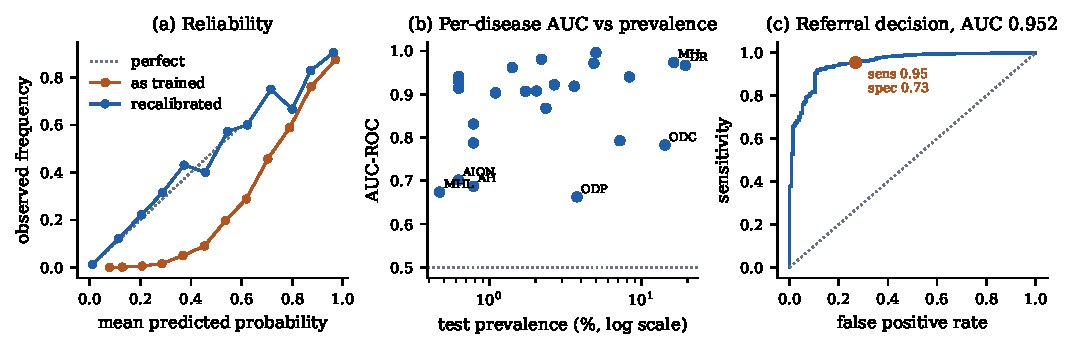
\includegraphics[width=\textwidth]{fig2_evidence.pdf}
    \caption{(a) Reliability on the test split before and after per-class Platt scaling; the
    as-trained curve sits far below the diagonal, which is over-confidence. (b) Per-disease AUC
    against test prevalence, log scale; the weakest classes are the rarest. (c) ROC for the
    referral decision, with the validation-fitted high-sensitivity operating point marked.}
    \label{fig:evidence}
\end{figure*}

\subsection{Effect of 8-Bit Quantisation}
Table~\ref{tab:quant} compares full and 8-bit precision directly on the same 640 test images with
identical CPU threading, replacing the previous unsupported claim of negligible loss. The claim
holds for ranking and fails for retrieval: macro AUC is unchanged at 0.873 against 0.872, but
macro AUPRC falls from 0.357 to 0.346, a 3.1\% relative loss concentrated in the rare classes
whose positive examples are already scarce. At the deployed operating point the quantised model is
slightly more permissive, catching eight more true positives at the cost of 218 additional false
alarms. Two practical points follow. First, a screening system should be re-thresholded after
quantisation rather than inheriting the full-precision thresholds, because quantisation shifts the
operating point even when it preserves the ranking. Second, dynamic quantisation is a storage
optimisation, not a speed one for this architecture: it cuts the exported model by 74.7\% but
reduces CPU latency by only 4\%, because PyTorch dynamic quantisation compresses linear weights
while the attention matrix products that dominate a ViT-L forward pass stay in floating point. The
latency benefit in deployment comes instead from the distilled MobileNetV3 student, which runs in
102\,ms per image at 5.4\,MB and agrees with its own FP32 export on 99.6\% of binary decisions.

\begin{table}[!t]
\centering
\caption{Effect of 8-bit dynamic quantisation on the reference model, on the same 640 test images
with identical CPU threading, so accuracy, size and latency are directly comparable. The deployed
on-device student compresses further, from 20.8\,MB to
5.4\,MB ONNX ($-$73.8\%), agreeing
with its FP32 export on 99.6\% of binary decisions at
$\tau{=}0.5$ and running at 102\,ms median per image.}
\label{tab:quant}
\scriptsize
\setlength{\tabcolsep}{3.5pt}
\begin{tabular}{lrccccr}
\toprule
Precision & MB & AUC & AUPRC & Sens. & PPV & ms/img \\
\midrule
FP32 & 1224 & 0.872 & 0.357 & 0.591 & 0.114 & 434 \\
INT8 dynamic & 310 & 0.873 & 0.346 & 0.610 & 0.106 & 418 \\
\midrule
Change & $-$74.7\% & +0.002 & -0.011 & +0.018 & -0.008 & $-$4\% \\
\bottomrule
\end{tabular}
\end{table}


\subsection{Faithfulness of the Explanations}
Table~\ref{tab:explain} reports the deletion/insertion test~\cite{rise2018} on 60 confidently
detected true positives, against a random-saliency control on the same images. Both attribution
methods pass the deletion test: removing the regions they highlight degrades the target
probability significantly faster than removing random regions (Grad-CAM $p{=}0.029$, Integrated
Gradients $p{=}0.008$, one-sided Wilcoxon). Neither passes the insertion test, where both are
statistically indistinguishable from random. The maps therefore identify regions the model uses,
but they do not identify a region set sufficient to reproduce the prediction, and the flat
insertion curves are a direct consequence of the calibration problem: predicted probabilities
never fall below 0.064, so revealing evidence has little room to move them. We accordingly
present the maps as attention hints requiring clinician verification, not as standalone evidence.
The narrative layer is audited separately for probability infidelity, omission of detected
findings, and unsupported escalation of urgency.

\begin{table}[!t]
\centering
\caption{Faithfulness of the explainability layer on 60 confidently detected true
positives. Deletion AUC is better when lower, insertion AUC when higher; $p$-values are one-sided
Wilcoxon signed-rank tests against the random-saliency control on the identical images.
Narrative layer ($n{=}24$ reports from the distilled narrator that always generates and never omits a detected finding): probability infidelity 0\% (95\% CI 0\%--14\%), finding omission 0\%, unsupported severity escalation 21\% (95\% CI 9\%--40\%).}
\label{tab:explain}
\scriptsize
\setlength{\tabcolsep}{3.5pt}
\begin{tabular}{lcccc}
\toprule
Attribution & Del.\ AUC & vs.\ rand. & Ins.\ AUC & vs.\ rand. \\
\midrule
Grad-CAM & 0.913 & $p=0.029$ & 0.926 & $p=0.996$ \\
Integrated Grad. & 0.861 & $p=0.008$ & 0.943 & $p=0.590$ \\
Random (control) & 0.946 & -- & 0.943 & -- \\
\bottomrule
\end{tabular}
\end{table}


\subsection{Referral Triage and What the Knowledge Graph Adds}
Per-disease multi-label metrics understate the system, because the output a primary-care operator
acts on is a single referral decision. Scored against the RFMiD \texttt{Disease\_Risk} flag, the
maximum class probability reaches an AUC of 0.952 (95\% CI 0.932--0.968) and an AUPRC of 0.986. At
the validation-fitted high-sensitivity operating point, test sensitivity is 0.955 and specificity
0.731, missing 23 of 506 positive images.

The knowledge graph's measurable contribution is here, not in classification accuracy. Its
co-occurrence rules almost never fire on the retained label set, because most of the partner
conditions they encode are among the 21 classes dropped for having too few training examples;
claiming a macro-F1 improvement from the graph, as the previous draft did, is not supportable. Its
referral-priority rules, however, do stratify risk monotonically once the thresholds are
non-degenerate: under the sensitivity-targeted policy the graph routes 84.5\% of images to
\textsc{urgent} (86.9\% of which carry pathology), 10.8\% to \textsc{routine} (47.8\%), and 4.7\%
to \textsc{follow-up} (10.0\%). Under the shipped thresholds the same rules classify 100\% of
images as \textsc{urgent} and carry no information at all, which is a further consequence of the
calibration failure.

\subsection{From Benchmark to Clinic}
Table~\ref{tab:prevalence} is the reason this paper does not claim clinical readiness. RFMiD is an
enriched research corpus in which 79\% of test images carry pathology. Holding the measured
sensitivity and specificity fixed and varying only prevalence, PPV falls from 0.931 on the
benchmark to 0.470 at 20\% prevalence and 0.158 at 5\%, while roughly 30\% of all screened
patients would still be referred. A screening programme sized on the benchmark PPV would
therefore under-provision its referral pathway by a factor of three or more. Negative predictive
value moves the other way, exceeding 0.99 at low prevalence, which is the property a
rule-out triage tool most needs.

\begin{table}[!t]
\centering
\caption{Why a benchmark result is not a clinical result. The referral operating point is held
fixed at the measured test sensitivity 0.955 and specificity
0.731; only the prevalence of the screened population changes. RFMiD is an
enriched research corpus, so its positive rate is far above any primary-care caseload.}
\label{tab:prevalence}
\scriptsize
\setlength{\tabcolsep}{3.5pt}
\begin{tabular}{lrccr}
\toprule
Population & Prev.\ (\%) & PPV & NPV & Refer (\%) \\
\midrule
RFMiD test (as measured) & 79 & 0.931 & 0.810 & 81 \\
\midrule
Projected at 30\% prev. & 30 & 0.604 & 0.974 & 47 \\
Projected at 20\% prev. & 20 & 0.470 & 0.985 & 41 \\
Projected at 10\% prev. & 10 & 0.283 & 0.993 & 34 \\
Projected at 5\% prev. & 5 & 0.158 & 0.997 & 30 \\
\bottomrule
\end{tabular}
\end{table}


\section{Discussion and Limitations}

We state concretely that benchmark results on international corpora cannot be interpreted as demonstration
of clinical efficacy in Uganda. RFMiD reflects predominantly South Asian demographics imaged on
table-top hospital fundus cameras. Zero Ugandan patient images were evaluated; hence, findings cannot
guarantee robustness across local retinal pigmentation, systemic comorbidities (e.g., HIV microangiopathy),
or handheld smartphone-adapted cameras used in district health centres. Our prevalence transfer model
(Section~V-H) quantifies the referral burden shift; optical distribution shifts remain unmeasured.

Three methodological constraints bound our claims. First, rare categories have limited statistical
power: 21 of 45 RFMiD labels were dropped for having fewer than 10 training positives, and conditions
with fewer than 20 evaluation positives exhibit wide bootstrap intervals. Second, the clinical knowledge
graph (Section~\ref{sec:kg}) is curated from published evidence but lacks independent ophthalmologist
panel review. Third, ablation arms share a standardized 15-epoch schedule, bounding relative contributions
rather than ceiling performance.

Clinical translation requires prospective multi-centre trials in Ugandan district facilities against
local ophthalmologist reference standards. Uganda National Drug Authority clearance, Data Protection
and Privacy Act (2019) compliance, ISO 13485 quality systems, and Good Machine Learning Practice alignment
remain prerequisites. An interactive demonstration is hosted at \url{https://landwind22-retinal-screening.hf.space}
as a workflow prototype, not a cleared device.

\section{Conclusion}

We evaluated OptiscanAI on the held-out RFMiD test split and report what the evidence supports.
Discrimination is strong (macro AUC 0.872; referral triage AUC 0.952), yet ablation reveals that retinal
foundation pretraining primarily confers parameter efficiency, while a fully fine-tuned ImageNet transformer
attains higher rare-class retrieval (AUPRC 0.472 vs 0.392). The shipped threshold policy is recall-prioritising
and silences five classes due to severe probability over-confidence (ECE 0.209); rank-preserving Platt scaling
resolves this failure mode (ECE 0.003). Attribution maps pass deletion but fail insertion fidelity testing.
Crucially, transferring triage operating points to primary-care prevalence cuts PPV by over half. We frame
this study as benchmark evidence and deployment analysis, with local prospective validation the essential
next step.

\section*{Acknowledgments}
The authors express gratitude to the faculty and research leadership at Makerere University's College
of Computing and Information Sciences for technical counsel throughout this investigation. We acknowledge
the curators of the public RFMiD repository for releasing their annotated dataset to the research community.
Furthermore, we sincerely thank the anonymous conference reviewers; their insightful critiques concerning
class-specific metrics, modular attribution, and demographic framing directly informed this revised
camera-ready manuscript.


\footnotesize
\begin{thebibliography}{99}

\bibitem{who2019} World Health Organization, ``World report on vision,'' World Health
Organization, Geneva, Switzerland, Tech.\ Rep., 2019.

\bibitem{teo2021} Z.~L. Teo, Y.-C. Tham, M.~Yu, \emph{et al.},
``Global prevalence of diabetic retinopathy and projection of burden through 2045: Systematic
review and meta-analysis,'' \emph{Ophthalmology}, vol.~128, no.~11, pp.~1580--1591, 2021.

\bibitem{gulshan2016} V.~Gulshan, L.~Peng, M.~Coram, \emph{et al.}, ``Development and validation of a deep learning algorithm for detection of diabetic
retinopathy in retinal fundus photographs,'' \emph{JAMA}, vol.~316, no.~22, pp.~2402--2410, 2016.

\bibitem{beede2020} E.~Beede, E.~Baylor, F.~Hersch, \emph{et al.}, ``A human-centered evaluation of a deep learning system deployed in clinics for
the detection of diabetic retinopathy,'' in \emph{Proc.\ CHI Conf.\ Human Factors in Computing
Systems}, 2020, pp.~1--12.

\bibitem{wiens2019} J.~Wiens, S.~Saria, M.~Sendak, \emph{et al.}, ``Do no harm: A roadmap for responsible machine learning for health care,''
\emph{Nature Medicine}, vol.~25, no.~9, pp.~1337--1340, 2019.

\bibitem{rfmid2021} S.~Pachade, P.~Porwal, D.~Thulkar, \emph{et al.}, ``Retinal fundus multi-disease image dataset
(RFMiD): A dataset for multi-disease detection research,'' \emph{Data}, vol.~6, no.~2, p.~14,
2021.

\bibitem{vit2021} A.~Dosovitskiy, L.~Beyer, A.~Kolesnikov, \emph{et al.}, ``An image is worth $16\times16$ words: Transformers for image
recognition at scale,'' in \emph{Proc.\ Int.\ Conf.\ Learning Representations (ICLR)}, 2021.

\bibitem{retfound2023} Y.~Zhou, M.~A. Chia, S.~K. Wagner, \emph{et al.}, ``A foundation model for generalizable disease detection from retinal
images,'' \emph{Nature}, vol.~622, pp.~156--163, 2023.

\bibitem{lora2022} E.~J. Hu, Y.~Shen, P.~Wallis, \emph{et al.}, ``LoRA: Low-rank adaptation of large language models,'' in \emph{Proc.\ Int.\ Conf.\
Learning Representations (ICLR)}, 2022.

\bibitem{gradcam2017} R.~R. Selvaraju, M.~Cogswell, A.~Das, \emph{et al.},
``Grad-CAM: Visual explanations from deep networks via gradient-based localization,'' in
\emph{Proc.\ IEEE Int.\ Conf.\ Computer Vision (ICCV)}, 2017, pp.~618--626.

\bibitem{shap2017} S.~M. Lundberg and S.-I. Lee, ``A unified approach to interpreting model
predictions,'' in \emph{Advances in Neural Information Processing Systems (NeurIPS)}, vol.~30,
2017, pp.~4765--4774.

\bibitem{ig2017} M.~Sundararajan, A.~Taly, and Q.~Yan, ``Axiomatic attribution for deep
networks,'' in \emph{Proc.\ Int.\ Conf.\ Machine Learning (ICML)}, 2017, pp.~3319--3328.

\bibitem{rise2018} V.~Petsiuk, A.~Das, and K.~Saenko, ``RISE: Randomized input sampling for
explanation of black-box models,'' in \emph{Proc.\ British Machine Vision Conf.\ (BMVC)}, 2018.

\bibitem{focal2017} T.-Y. Lin, P.~Goyal, R.~Girshick, \emph{et al.}, ``Focal loss for
dense object detection,'' in \emph{Proc.\ IEEE Int.\ Conf.\ Computer Vision (ICCV)}, 2017,
pp.~2980--2988.

\bibitem{asl2021} T.~Ridnik, E.~Ben-Baruch, N.~Zamir, \emph{et al.}, ``Asymmetric loss for multi-label classification,'' in \emph{Proc.\ IEEE Int.\
Conf.\ Computer Vision (ICCV)}, 2021, pp.~82--91.

\bibitem{guo2017} C.~Guo, G.~Pleiss, Y.~Sun, \emph{et al.}, ``On calibration of modern
neural networks,'' in \emph{Proc.\ Int.\ Conf.\ Machine Learning (ICML)}, 2017, pp.~1321--1330.

\bibitem{claim2024} A.~S. Tejani, M.~E. Klontzas, A.~A. Gatti, \emph{et al.}, ``Checklist for Artificial Intelligence in Medical Imaging (CLAIM): 2024
update,'' \emph{Radiology: Artificial Intelligence}, vol.~6, no.~4, e240300, 2024.

\bibitem{tripodai2024} G.~S. Collins, K.~G.~M. Moons, P.~Dhiman, \emph{et al.}, ``TRIPOD+AI statement: Updated guidance for reporting clinical
prediction models that use regression or machine learning methods,'' \emph{BMJ}, vol.~385,
e078378, 2024.

\bibitem{futureai2025} K.~Lekadir, A.~Frangi, A.~R. Porras, \emph{et al.}, ``FUTURE-AI: International consensus guideline for trustworthy and
deployable artificial intelligence in healthcare,'' \emph{BMJ}, vol.~388, e081554, 2025.

\end{thebibliography}

\end{document}
